\documentclass{article}
\usepackage{geometry}
\usepackage{graphicx}
\usepackage{amsmath}
\usepackage{algorithm}
\usepackage{algpseudocode}
\usepackage{dsfont}
\usepackage{amssymb}
\usepackage{multicol}
\usepackage{wrapfig}
\usepackage{tipa}
\geometry{
a4paper,
right=10mm,
left=10mm,
top=10mm,
bottom=10mm,	
}

\begin{document}

\pagenumbering{gobble}

\begin{center}
\textbf{\Large HOMEWORK 3 : CS771} \\
\textit{\large Jayant Agrawal}         14282
\end{center}
\section{Problem 1- Kernel Perceptron}
\begin{figure}[h!]
\centering
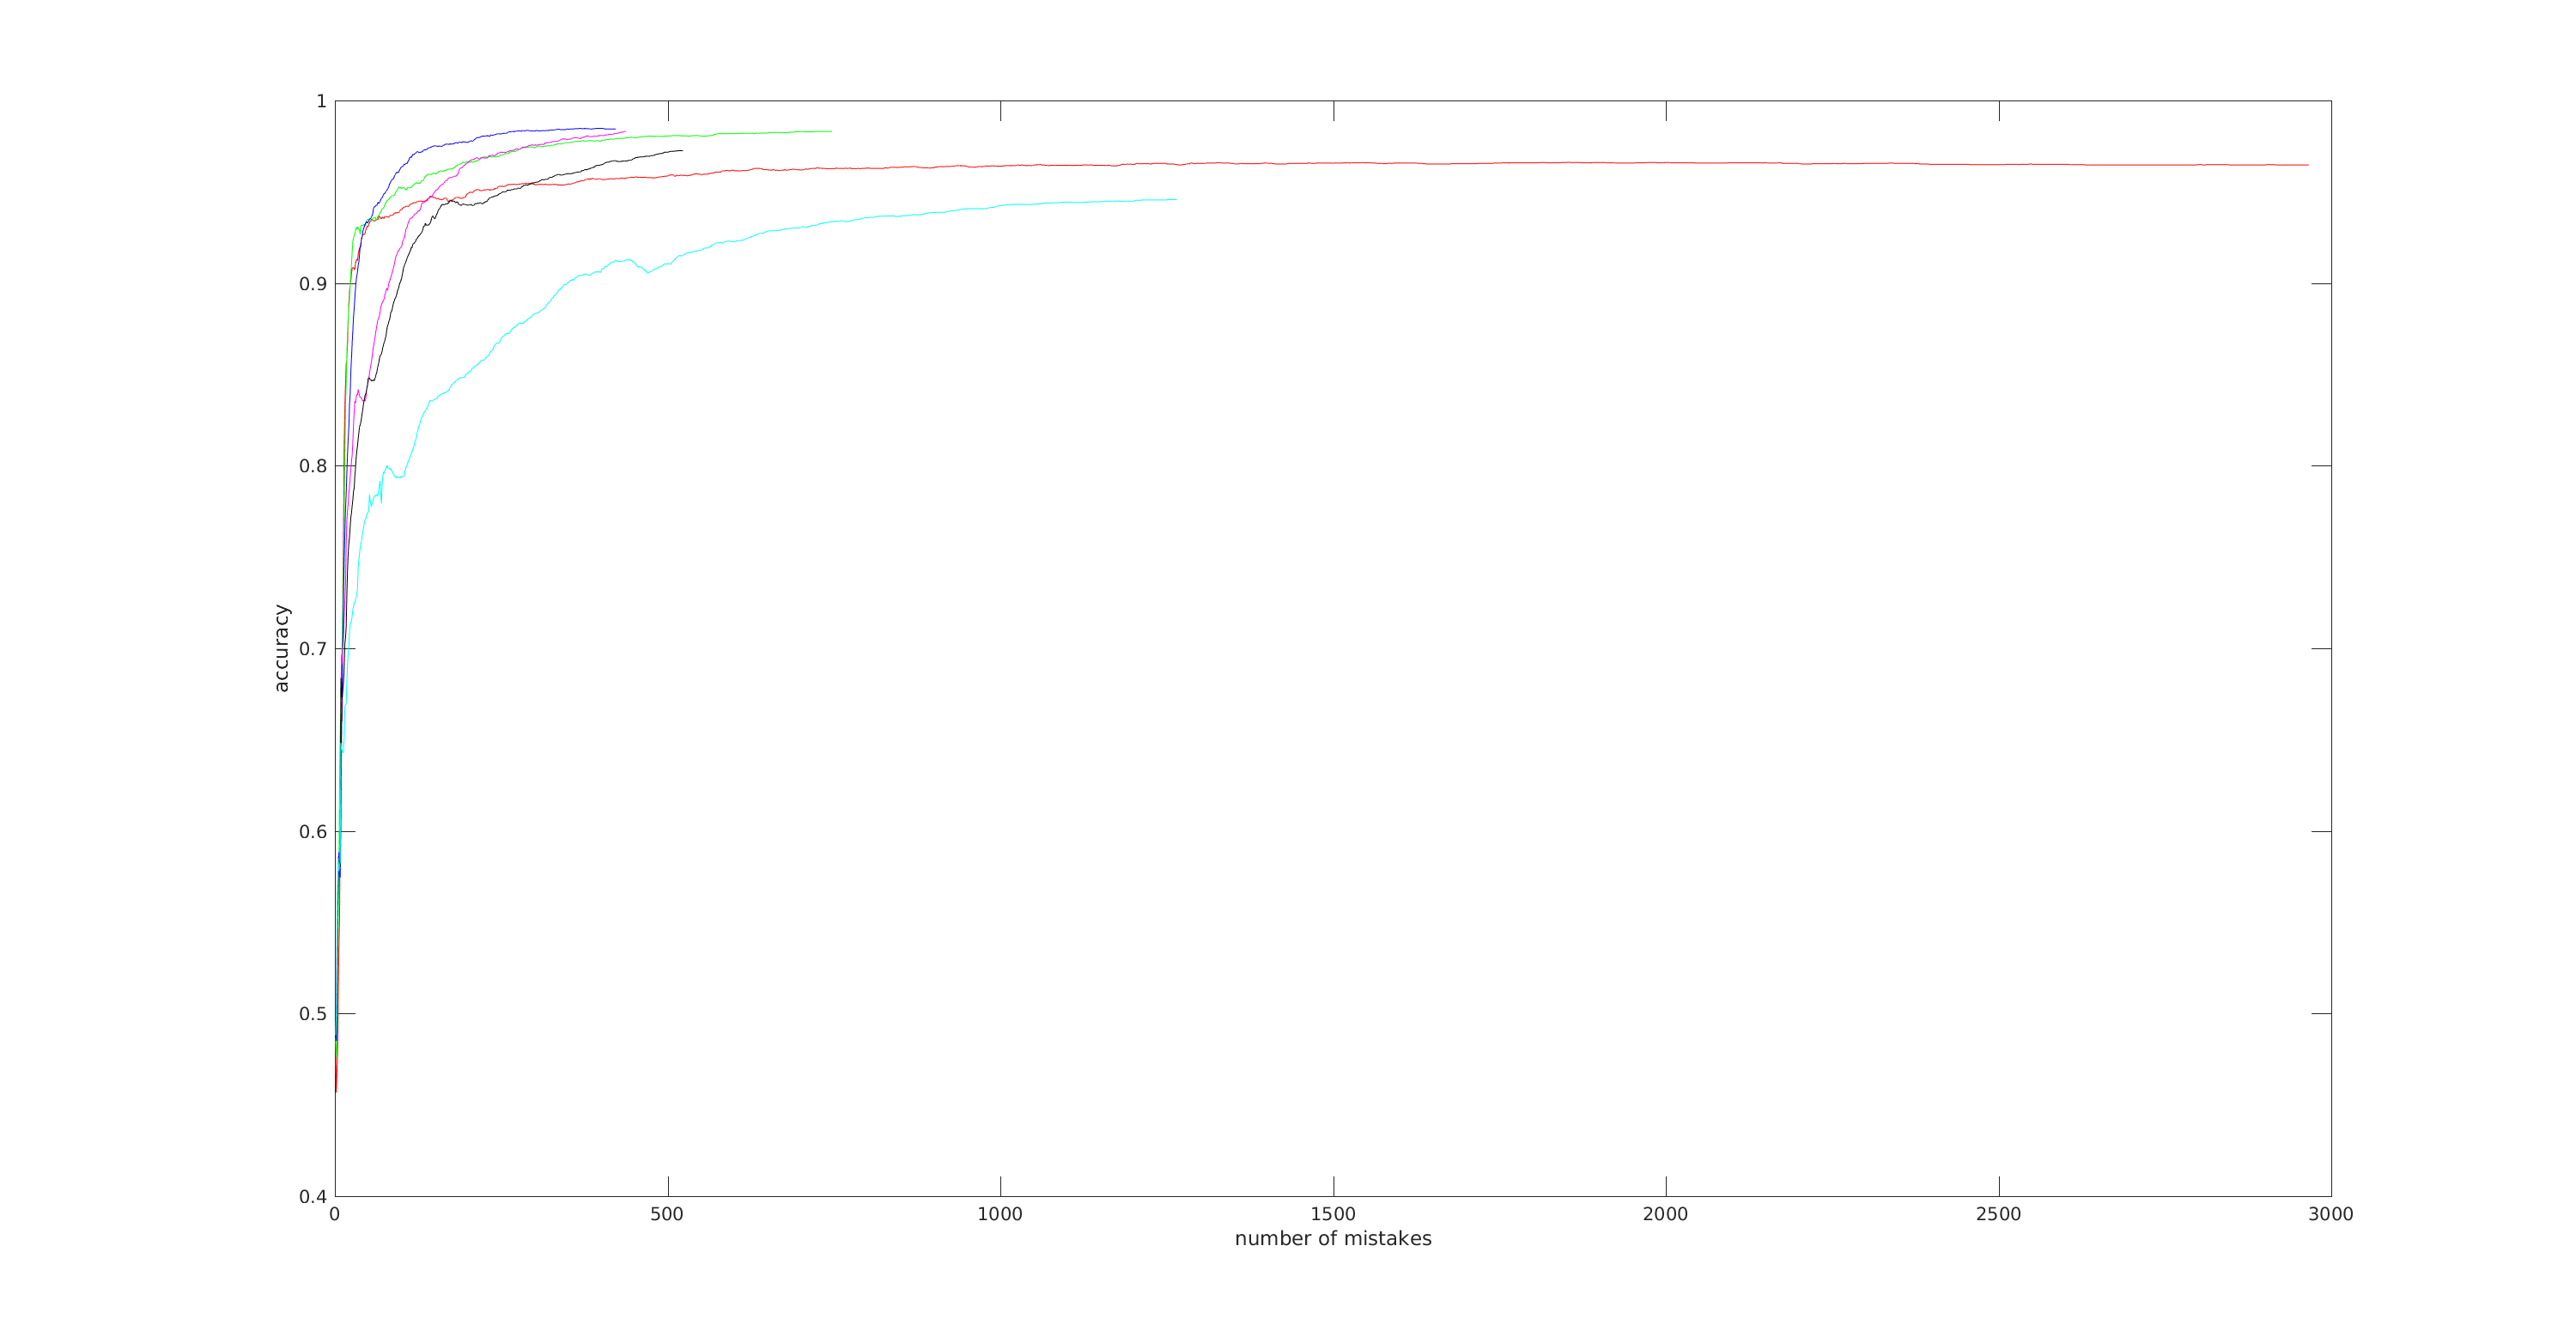
\includegraphics[width=1\columnwidth]{acc_avg.png}
\caption{Red = 1, Green = 2, Blue = 4, Pink = 8, Black = 10, Cyan = 20}
\label{acc}
\end{figure}
\begin{center}
\emph{Kernel with Test Accuracy: }4 (Blue)\\ 
\emph{Kernel with Minimum Mistakes: }4 (Blue) 
\end{center}

\section{Problem 2- Matrix Factorization}
\begin{figure}[h!]
\centering
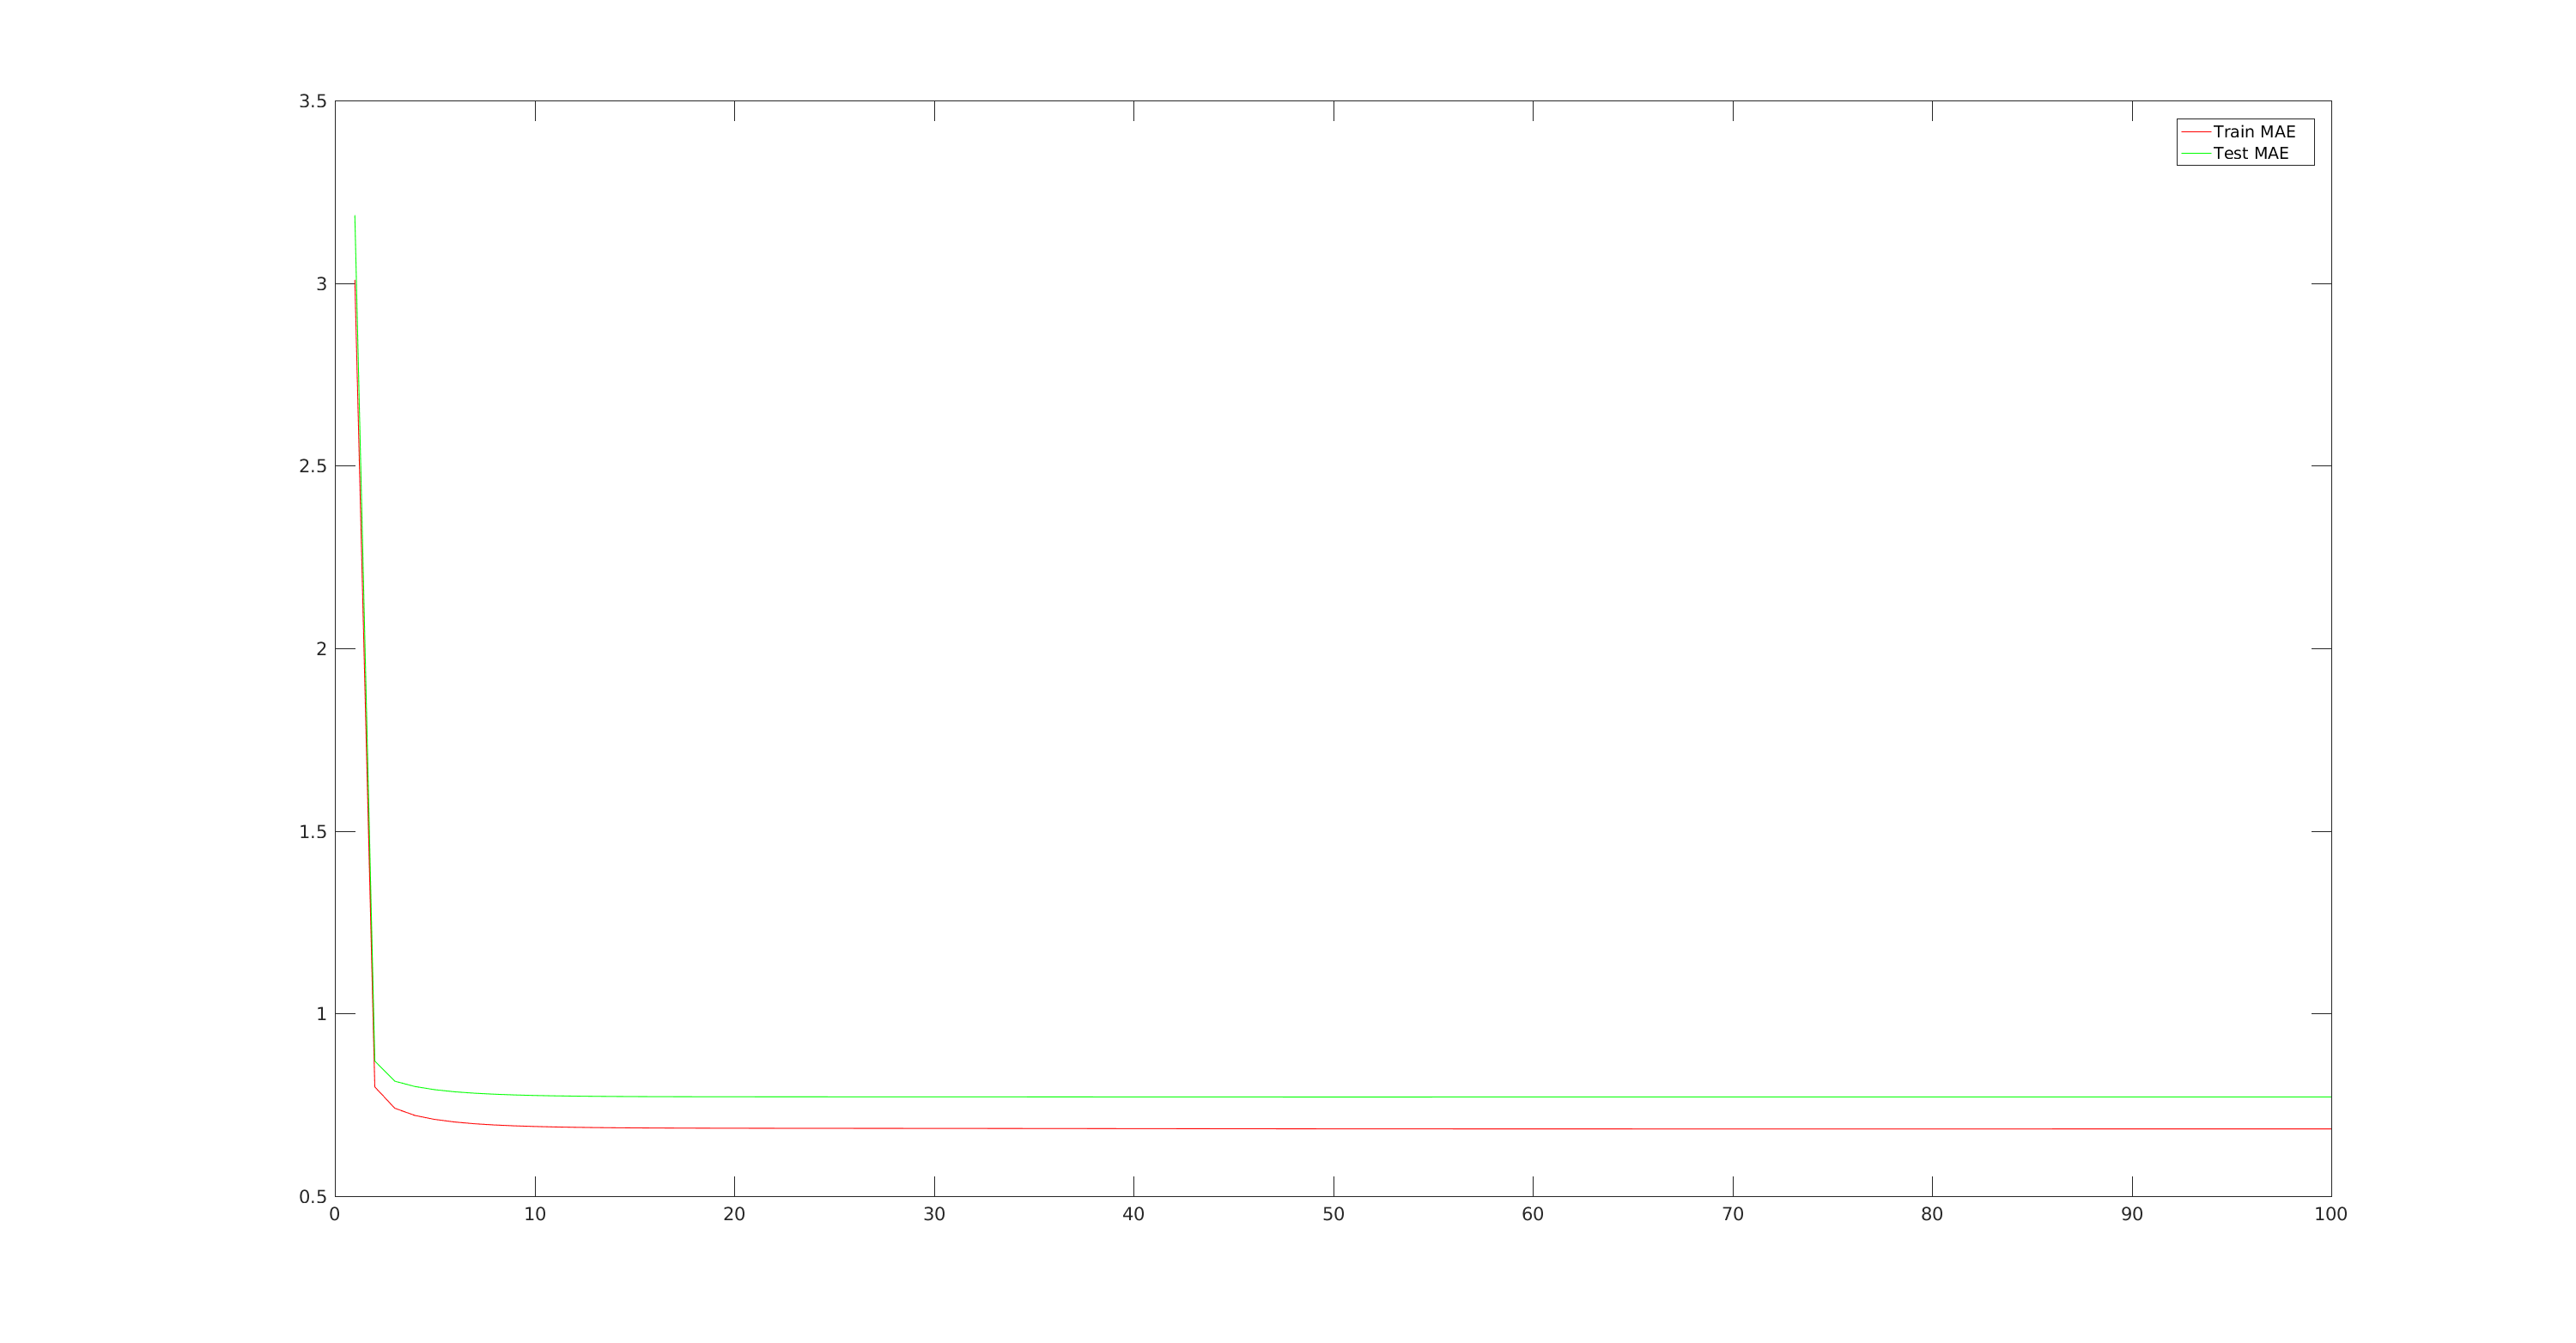
\includegraphics[width=1\columnwidth]{mae2.png}
%\caption{Red = 1, Green = 2, Blue = 4, Pink = 8, Black = 10, Cyan = 20}
\label{mae}
\end{figure}

\section{Problem 3 - GMM }
Assuming that gaussians have a shared spherical diagonal covariance matrix $\sigma^2\text{\textbf{I}}_D$.  Section \ref{sig} contains derivation for $\sigma^2$.
\subsection{Expression for $\sigma^2$}
\label{sig}
Expected Complete data Log-Likelihood ($\mathcal{L}$) for this model can be written as:
$$\mathcal{L} = \sum_{n=1}^N \sum_{k=1}^K \mathds{E}[z_{nk}][log\pi_k + log \mathcal{N}(x_n | \mu_k, \Sigma))]$$
where $\mathds{E}[z_{nk}] = \frac{\pi_k \mathcal{N}(x_n| \mu_k, \Sigma)}{\sum_{l=1}^K \mathcal{N}(x_n| \mu_k, \Sigma)}$ and $\Sigma = \sigma^2\textbf{I}_D$. Also, $\sum_{k=1}^K \mathds{E}[z_{nk}]=1$. \\ \\
Using $\mathds{E}[z_{nk}] = \gamma_{nk}$, taking derivative w.r.t $\mu_k$ and setting it to zero $\forall k = 1,...K $(The derivation for $u_k$ is similar to the general case shown in class except that $\Sigma_k$ is replaced by $\Sigma$), we get :
$$ \frac{\partial \mathcal{L}}{\partial \mu_k} = \frac{\partial}{\partial \mu_k} \sum_{n=1}^N \gamma_{nk} log \mathcal{N}(x_n | \mu_k, \Sigma) = 0 $$
We get the following expression for $\mu_k$, as shown in the note and lectures:
$$\mu_k = \frac{1}{N_k}\sum_{n=1}^N \gamma_{nk}x_n$$
where $N_k = \sum_{n=1}^N \gamma_{nk}$. \\ \\
Now, taking derivative of $\mathcal{L}$ w.r.t $\Sigma$:
\begin{equation*}
\begin{aligned}
\frac{\partial \mathcal{L}}{\partial \Sigma} &= \frac{\partial}{\partial \Sigma} \sum_{n=1}^N \sum_{k=1}^K \gamma_{nk}[ log \pi_k + log \mathcal{N}(x_n | \mu_k, \Sigma)] \\
&= \sum_{n=1}^N \sum_{k=1}^K \gamma_{nk} \frac{\partial}{\partial \Sigma} log \mathcal{N}(x_n | \mu_k, \Sigma) \\
\end{aligned}
\end{equation*}
Now, proceeding as shown in the note, Consider $log \mathcal{N}(x_n | \mu_k, \Sigma)$ :
\begin{equation*}
\begin{aligned}
log \mathcal{N}(x_n | \mu_k, \Sigma) &\propto - \frac{1}{2}log|\Sigma| - \frac{1}{2}(x_n- \mu_k)^T\Sigma^{-1}(x_n-\mu_k)\\
&= \frac{1}{2}log|\Sigma^{-1}| - \frac{1}{2}(x_n- \mu_k)^T\Sigma^{-1}(x_n-\mu_k) \\
&= \frac{1}{2}log|\Sigma^{-1}| - \frac{1}{2}tr[(x_n- \mu_k)(x_n-\mu_k)^T\Sigma^{-1} ]\\
\end{aligned}
\end{equation*}
Taking derivatives wrt. $\Sigma^{-1}$ (instead of $\Sigma$):
\begin{equation*}
\begin{aligned}
\sum_{n=1}^N\sum_{k=1}^K \gamma_{nk}\frac{\partial}{\partial \Sigma^{-1}}[ \frac{1}{2}log|\Sigma^{-1}| - \frac{1}{2}tr[(x_n- \mu_k)(x_n-\mu_k)^T\Sigma^{-1}]] &= 0\\
\sum_{n=1}^N\sum_{k=1}^K \gamma_{nk} [\Sigma - (x_n- \mu_k)(x_n-\mu_k)^T ] &=0 \\
\end{aligned}
\end{equation*}
Thus, we get the following expression for $\Sigma = \sigma^2\textbf{I}$:
\begin{equation*}
\begin{aligned}
\Sigma &= \frac{1}{\sum_{n=1}^N\sum_{k=1}^K \gamma_{nk}} \sum_{n=1}^N\sum_{k=1}^K \gamma_{nk}(x_n- \mu_k)(x_n-\mu_k)^T \\
\end{aligned}
\end{equation*}
Comparing the diagonal entries from the two sides, we get:
$$\sigma^2 = \frac{\sum_{n=1}^N (x_n^Tx_n - \sum_{k=1}^K \gamma_{nk}\mu_k^T\mu_k)}{D*\sum_{n=1}^N\sum_{k=1}^K \gamma_{nk}}$$
$$\sigma^2 = \frac{\sum_{n=1}^N x_n^Tx_n - \sum_{k=1}^KN_{k}\mu_k^T\mu_k}{D*\sum_{k=1}^K N_{k}}$$
$$\sigma^2 = \frac{\sum_{n=1}^N x_n^Tx_n - \sum_{k=1}^KN_{k}\mu_k^T\mu_k}{D*N}$$
\newpage
\subsection{Results}
\subsubsection{Fig 1}
\begin{figure}[h!]
\centering
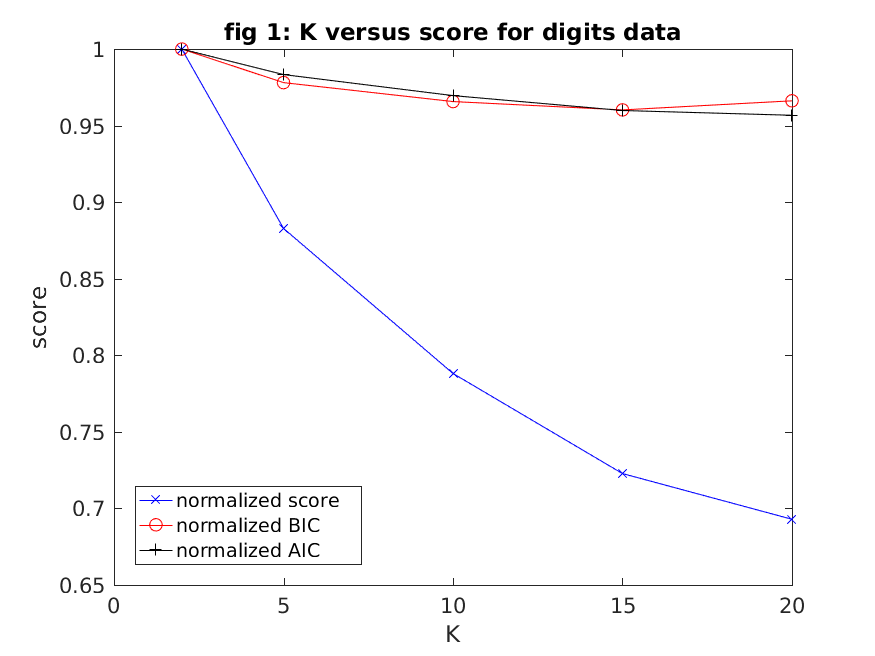
\includegraphics[width=0.9\columnwidth]{results3/1.png}
\label{1}
\end{figure}
Incomplete Data Likelihood is given by: $p(x_n)$, whereas complete data likelihood is given by $p(x_n,z_n)$. There is no significant difference between the two. Yes, the CLL's seem to roughly converge to the same value across all runs.
\subsubsection{Fig 2}
\begin{figure}[h!]
\centering
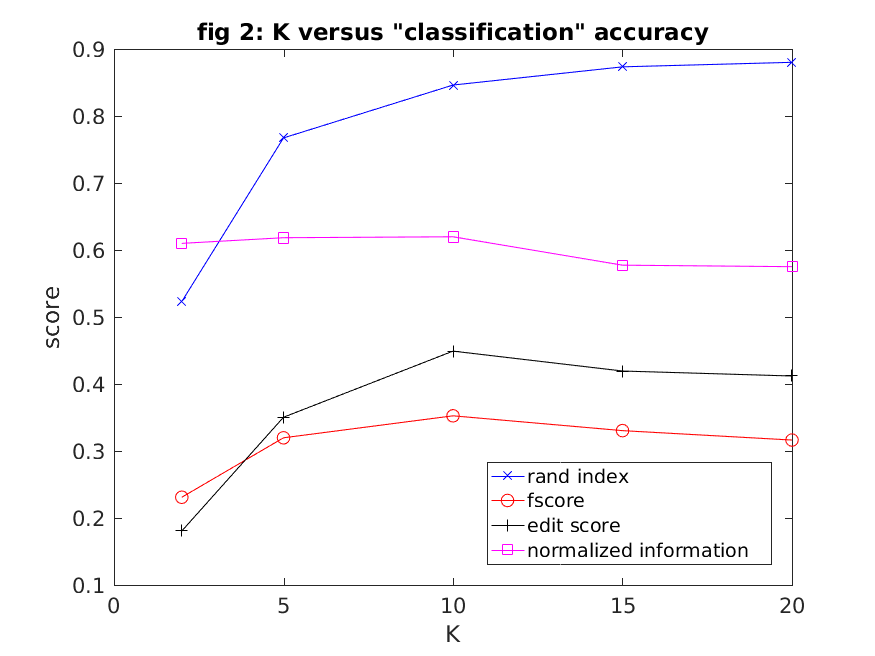
\includegraphics[width=0.35\columnwidth]{results3/2.png}
\label{2}
\end{figure}
The graph attains a minima at 20. Yes, this makes sense, since the lower the BIC, the better it is. If the clusters are increased beyond an optimum point, the BIC score increases.
\subsubsection{Fig 3-9}
\textbf{Fig 3(2 clusters)-4(5 clusters) }
\begin{figure}[h!]
\centering
\begin{multicols}{2}
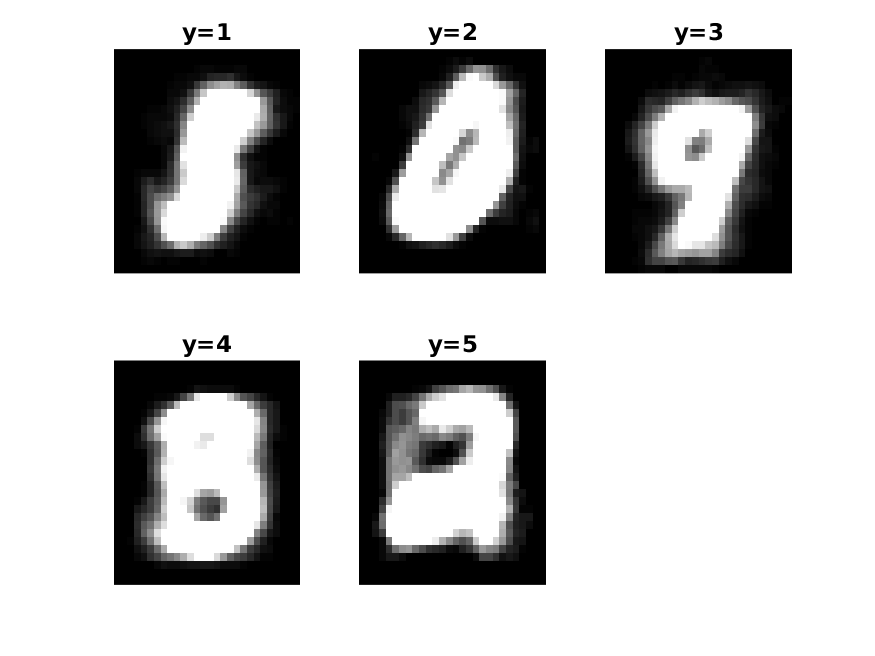
\includegraphics[width=1\columnwidth]{results3/3.png}
\label{3}

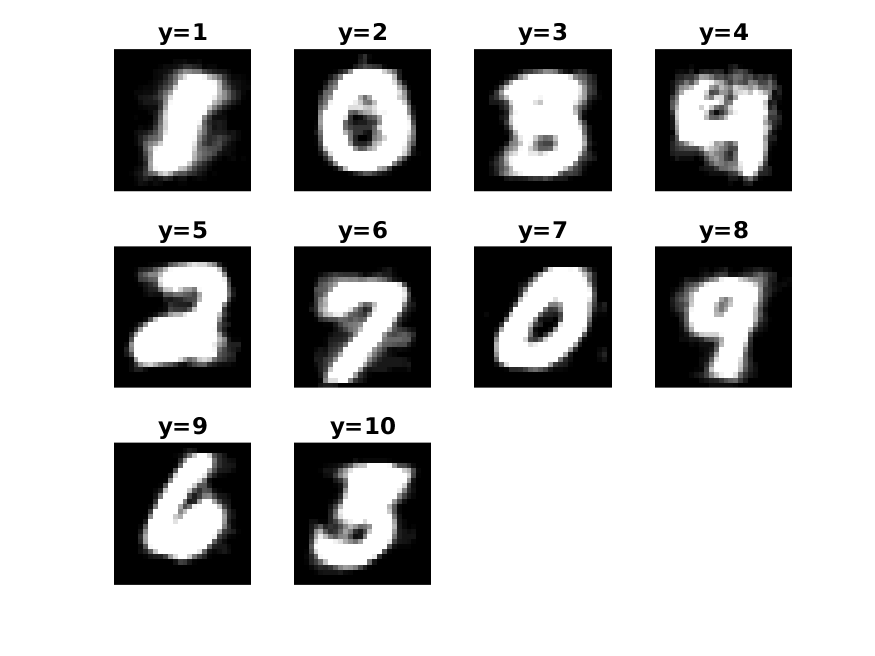
\includegraphics[width=1\columnwidth]{results3/4.png}
\label{4}
\end{multicols}
\end{figure}
\newpage
\textbf{Fig 5(10 clusters)}
\begin{figure}[h!]
\centering
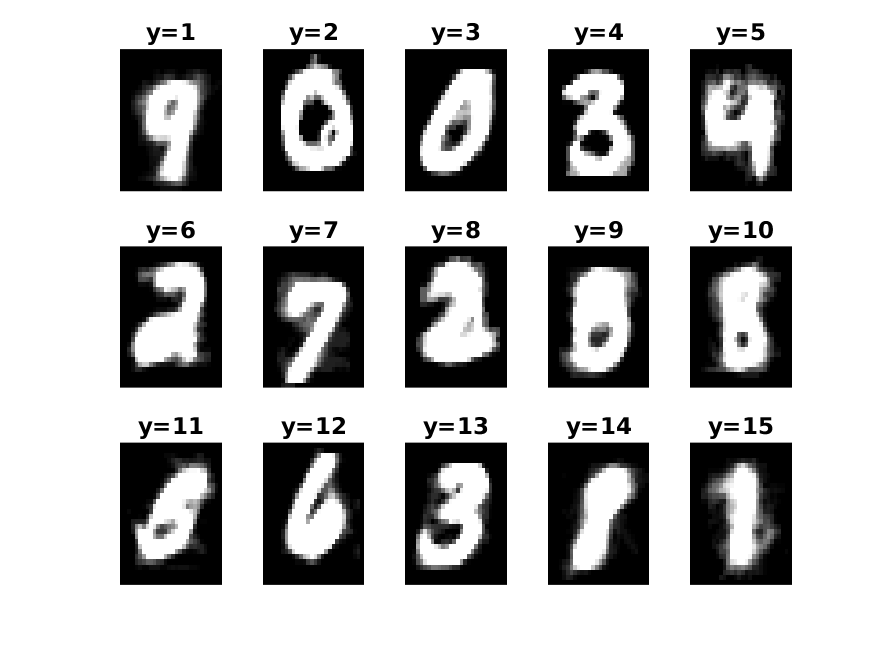
\includegraphics[width=0.8\columnwidth]{results3/5.png}
\label{5}
\end{figure}
\newline
\textbf{Fig 6(15 clusters)}
\begin{figure}[h!]
\centering
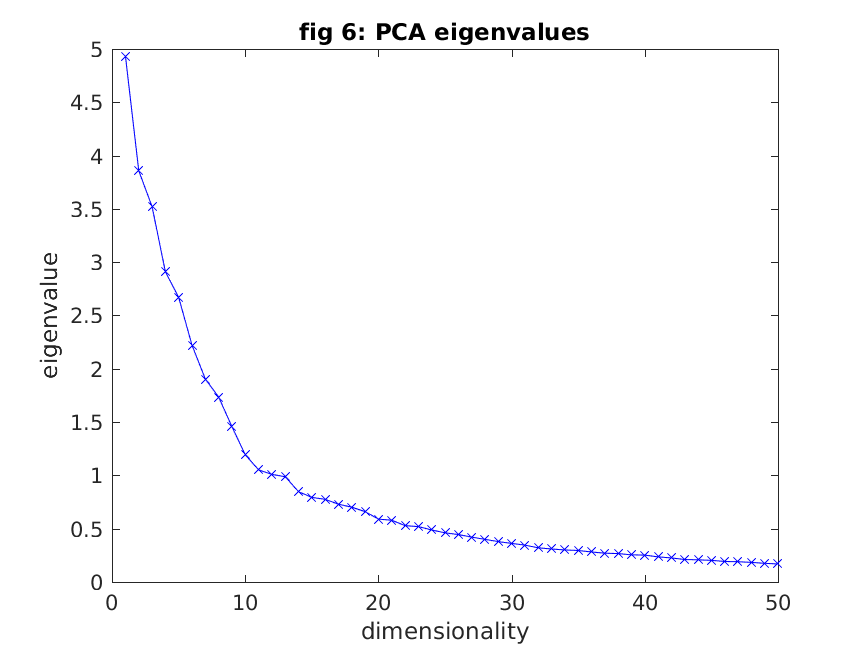
\includegraphics[width=0.8\columnwidth]{results3/6.png}
\label{6}
\end{figure}
\newline
\textbf{Fig 7(20 clusters)}
\begin{figure}[h!]
\centering
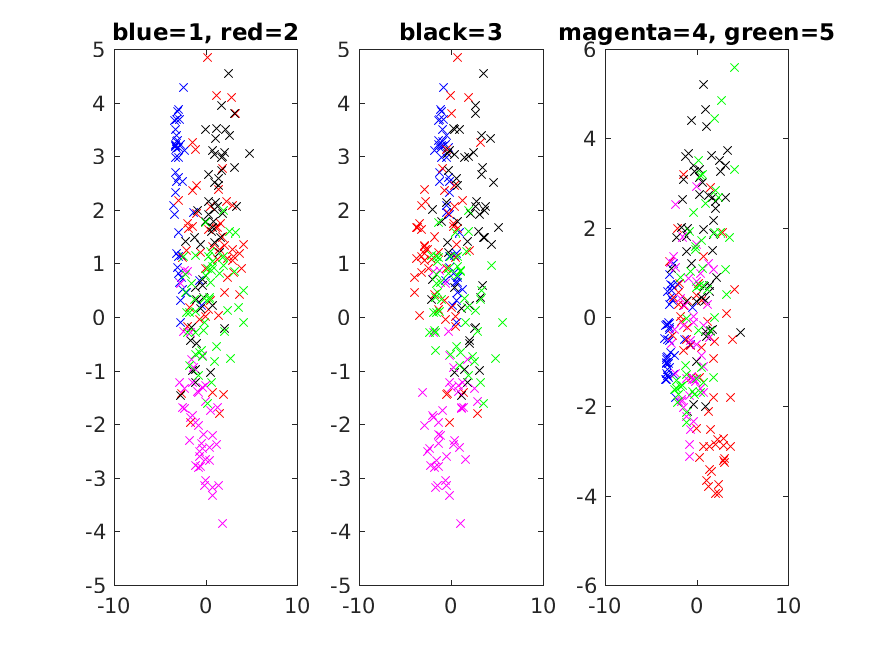
\includegraphics[width=0.8\columnwidth]{results3/7.png}
\label{7}
\end{figure}
\newpage
\textbf{Fig 8(25 clusters)}
\begin{figure}[h!]
\centering
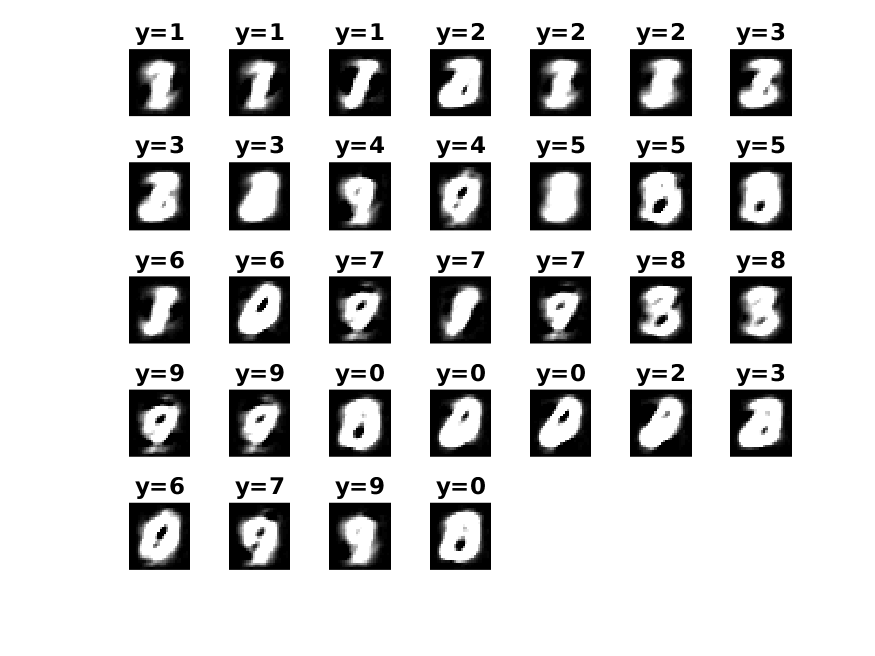
\includegraphics[width=1\columnwidth]{results3/8.png}
\label{8}
\end{figure}
\newline
\textbf{Fig 9(30 clusters)}
\begin{figure}[h!]
\centering
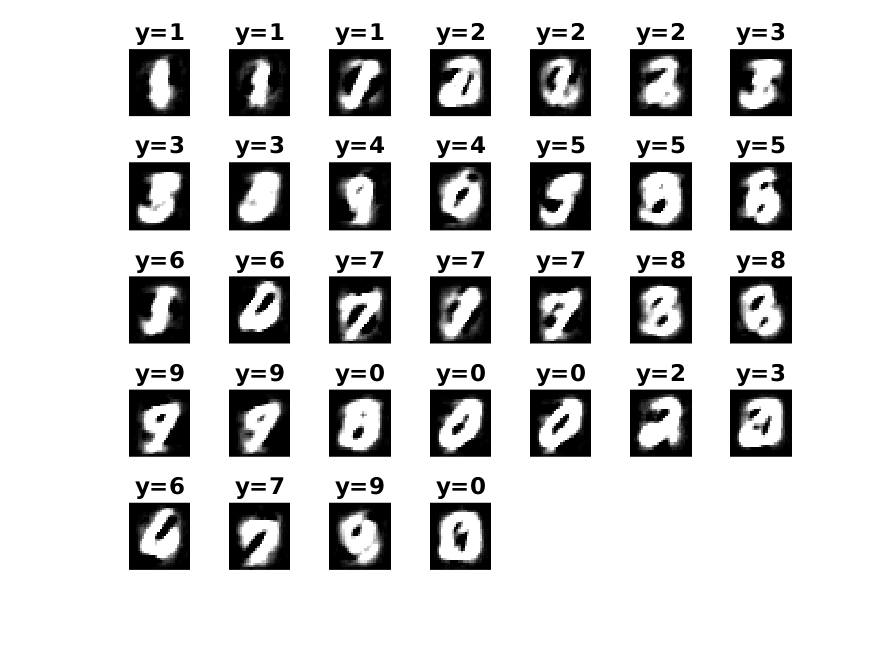
\includegraphics[width=1\columnwidth]{results3/9.png}
\label{9}
\end{figure}

'Real digits' start appearing at the cluster size of 10 and they become clear enough at the cluster size of 20. Also, at 20 clusters, atleast one example from each digit can be seen. The blurry cases are mixtures of digits which appear similar (3 and 8), in other words, the digits with closer means appear blurry in some cases. Though, there does not seem to be a significant pattern between the quality of mean and pk values. However, clarity seems to improve with lower pk values, which should happen since pk are mixture weights.

\section{Problem 4 - EM for Poisson Mixture Model}
As shown in the problem statement: complete data likelihood for each point n is as follows:
$$p(k,z |  \lambda, \pi) = \prod_{n=1}^N\prod_{l=1}^L\Bigg[\pi_l\prod_{m=1}^M Poisson(k_{n,m}|\lambda_l)\Bigg]^{\textbf{1}[z_n=l]}$$
Thus, the \textbf{complete data log likelihood} for the model is as follows:
$$ log\big(p(k,z |  \lambda, \pi)\big) = \sum_{n=1}^N\sum_{l=1}^Lz_{nl}\Bigg[\log(\pi_l)+ log\bigg(\prod_{m=1}^M Poisson(k_{n,m}|\lambda_l)\bigg)\Bigg]$$
where, $z_{nl}$ is 1 if $\textbf{1}[z_n=l]$, 0 otherwise(using the one-hot notation for $z_n$). \\ \\
\textbf{Estimating $z_{nl}$: }
\begin{equation*}
\begin{aligned}
\mathds{E}[z_{nl}] &= 0 \times p(z_{nl}=0|k_n) + 1 \times p(z_{nl} =1 |k_n) \\
\mathds{E}[z_{nl}] &= p(z_{nl} =1 |k_n) \\
&\propto  p(z_{nl}=1)p(k_n|z_{nl}=1)\\
\mathds{E}[z_{nl}] &\propto \pi_k \mathcal{N}(x_n | z_{nl}=1)
\end{aligned}
\end{equation*}
\textbf{Estimating $\lambda_l$} \\ \\
Expected Complete Data log-likelihood (taking $\mathds[z_{nl}] = \gamma_{nl}$) : 
$$ \mathcal{L} =  \sum_{n=1}^N\sum_{l=1}^L\gamma_{nl}\Bigg[\log(\pi_l)+ log\bigg(\prod_{m=1}^M Poisson(k_{n,m}|\lambda_l)\bigg)\Bigg] $$
Taking Derivative w.r.t $\lambda_l$.
\begin{equation*}
\begin{aligned}
\frac{\partial \mathcal{L}}{\partial \lambda_l} &=  \sum_{n=1}^N\gamma_{nl}\Bigg[\frac{\partial}{\partial \lambda_l}  log\bigg(\prod_{m=1}^M Poisson(k_{n,m}|\lambda_l)\bigg)\Bigg]  \\
\frac{\partial \mathcal{L}}{\partial \lambda_l} &=  \sum_{n=1}^N\gamma_{nl}\Bigg[\frac{\partial}{\partial \lambda_l} \bigg(\sum_{m=1}^Mlog\bigg( Poisson(k_{n,m}|\lambda_l)\bigg)\bigg)\Bigg]  \\
\frac{\partial \mathcal{L}}{\partial \lambda_l} &=  \sum_{n=1}^N\gamma_{nl}\Bigg[\frac{\partial}{\partial \lambda_l} \bigg(\sum_{m=1}^M k_{n,m}log(\lambda_l) - \lambda_l - log(k_{n,m}!) \bigg)\Bigg]  \\
\frac{\partial \mathcal{L}}{\partial \lambda_l} &=  \sum_{n=1}^N\gamma_{nl}\Bigg[\frac{\partial}{\partial \lambda_l} \bigg(\sum_{m=1}^M \frac{k_{n,m}}{\lambda_l} - 1 \bigg)\Bigg]  \\
\end{aligned}
\end{equation*}
Setting it to 0 :
$$\frac{\partial \mathcal{L}}{\partial \lambda_l} =  0 $$
\begin{equation*}
\begin{aligned}
\sum_{n=1}^N\gamma_{nl}\Bigg[\frac{\partial}{\partial \lambda_l} \bigg(\sum_{m=1}^M \frac{k_{n,m}}{\lambda_l} - 1 \bigg)\Bigg]  &= 0\\
\frac{1}{\lambda_l}\sum_{n=1}^N \gamma_{nl}\sum_{m=1}^M k_{n,m} &= \sum_{n=1}^N \gamma_{nl}M \\
\end{aligned}
\end{equation*}
$$\lambda_l = \frac{\sum_{n=1}^N \gamma_{nl}\sum_{m=1}^M k_{n,m}}{\sum_{n=1}^N \gamma_{nl}M} $$
\textbf{Estimating $\pi_l$: }\\ \\
Since $\sum_{l=1}^L\pi_l = 1$, the constrained optimization problem's objective (as shown in the note) is as follows:
$$\mathcal{L} = \sum_{n=1}^N\sum_{l=1}^L\gamma_{nl} log(\pi_l) + \alpha*(1- \sum_{l=1}^L\pi_l)$$
Taking Derivative w.r.t $\pi_l$:
\begin{equation*}
\begin{aligned}
\frac{\partial \mathcal{L}}{\partial \pi_l} &= \sum_{n=1}^N \frac{\gamma_{nl}}{\pi_l} - \alpha \\ 
\end{aligned}
\end{equation*}
Setting $\frac{\partial \mathcal{L}}{\partial \pi_l}  = 0$ :
$$\sum_{n=1}^N \frac{\gamma_{nl}}{\pi_l} - \alpha  = 0$$
$$\pi_l = \frac{\sum_{n=1}^N \gamma_{nl}}{\alpha}$$
Using the fact that $\sum_{l=1}^L\pi_l = 1$, we get :
$$\sum_{l=1}^L\frac{\sum_{n=1}^N\gamma_{nl}}{\alpha} = 1$$
$$\alpha = \sum_{n=1}^N\sum_{l=1}^L \gamma_{nl}$$
$$\alpha = N$$
Thus, using this value of $\alpha$ in the previous expression for $\pi_l$,
$$\pi_l = \frac{1}{N} \sum_{n=1}^N \gamma_{nl }$$

\section{Problem 5}
\subsection{Embeddings}
K-means gives a one-hot vector embedding($z_n$) for each $x_n$, which depicts the cluster to which $x_n$ belongs. GMM differs from K-means in a sense that it also gives the probability with which $x_n$ belongs to any cluster, also known as soft-clustering. The embedding learned by GMM can thus be seen as a probability vector. PCA, on the other hand, gives an efficient way to convert a D-dimensional vector of $x_n$ into a K-dimensional vector, where K<<D. The embedding learned by PCA can thus be seen as a compact representation of the original data point.

\subsection{Expectation Maximisation}
In general, the goal in the case of a generative model is to estimate parameters of the model that maximises the probability of the observed data. The most easy way to do this, is obviously, using MLE/MAP. But, in general, doing MLE in such models can be difficult because of the log-sum/integral(as shown in slides). In this case, we need Expectation Maximisation Algorithm. \\ \\
The core idea behind EM algorithm remains the same as in the case of the simple MLE/MAP, that is, maximise the probability of the observed data. Although, the EM algorithm maximises the Expectation of log probability instead of maximising the log-probability, it can be shown that the log probability is tightly lower bounded by expectation of log probabality. Thus, the parameters learned by the EM algorithm are very close to those that could have been learned by MLE/MAP (if possible). \\ \\
As shown in slide 13 of Lecture 17, the $\mathcal{L}$ curve touches the $log p(X|\theta)$ curve at the E-step. In the M-step, we compute the paramters that maximise the current $\mathcal{L}$ curve. Again, in the next E-step, the curve is changed to meet $log p(X|\theta)$ curve again. This continues untill a local maxima is reached. The algorithm thus, gives us parameter estimates which will be very close to the actual parameters that actually maximises the log probability.


\end{document}


